\documentclass[10pt,a4paper,hidelinks]{article}
\usepackage[utf8]{inputenc}
\usepackage[english]{babel}
\usepackage[T1]{fontenc}

\newcommand{\documentStatus}{DRAFT}


\usepackage{amsmath}
\usepackage{amsfonts}
\usepackage{amssymb}
\usepackage{graphicx}
\usepackage{lmodern}
\usepackage{tikz}
\usetikzlibrary{positioning}
\usetikzlibrary{shapes,snakes}
\usepackage{epigraph} 
\usepackage[left=2.5cm,
            right=2.5cm,
            top=2cm,
            bottom=2cm]{geometry}
\usepackage{setspace}
\usepackage{caption}
\usepackage{subcaption}
\usepackage{epigraph}
\usepackage{pdflscape}
\usepackage{pgfplots}

\usepackage{titlesec}
\usepackage{tcolorbox}
\usepackage{background}
\usepackage{url}
\usepackage[pdfauthor={Pierre Jézégou},
            pdftitle={ADS assignement},
            pdfsubject={Word games},
            pdfkeywords={}]{hyperref}
\usepackage{wrapfig}

\backgroundsetup{contents=\documentStatus, color=\watermarkColor}

\usepackage{fancyhdr}
\usepackage{textpos}
\usepackage{sectsty}
\usepackage{xcolor}

\setlength{\parindent}{0pt}

%%%%%%%%%%%%%%% Colors %%%%%%%%%%%%%%%
\subsectionfont{\color{fib_red}}
\subsubsectionfont{\color{fib_red}}
\renewcommand\fbox{\fcolorbox{black}{fib_red!20}}

\definecolor{fib_red}{RGB}{191,21,64}
\definecolor{fib_gray}{RGB}{111,111,111}
\definecolor{blue_upc}{RGB}{52,120,186}

\usepackage{listings}
\lstdefinestyle{mystyle}{
  backgroundcolor=\color{gray!10},
  stringstyle=\color{green!50!black},
  keywordstyle=\color{fib_red},
  numberstyle=\tiny\color{fib_gray},
  commentstyle=\color{blue_upc},
  basicstyle=\ttfamily\footnotesize,
  breakatwhitespace=false,         
  breaklines=true,                 
  captionpos=b,                    
  keepspaces=true,                 
  numbers=left,                    
  numbersep=5pt,                  
  showspaces=false,                
  showstringspaces=false,
  showtabs=false,                  
  tabsize=2
}

\lstset{style=mystyle}

\usepackage[Bjornstrup]{fncychap}
\newcommand{\watermarkColor}{red!10}


\onehalfspacing


\newcommand\VRule[1][\arrayrulewidth]{\vrule width #1}
\usepackage{xcolor,colortbl}

\newtcolorbox{mybox}[1]{
    arc=5pt,
    boxrule=0pt,
    colback=#1,
    width=\linewidth,
    halign=left,
}

\newenvironment{framed}[3]{
    \vspace*{0.5em}
    \begin{mybox}{#3!10}
        \textbf{#1}:\hfill \textit{#2}\\
        \hrule\vspace*{1em}
}
{\end{mybox}}

\newenvironment{exercise_description}[1]{
    \begin{framed}{Exercise description}{#1}{orange}
}
{\end{framed}}

\newenvironment{summary}{
    \begin{framed}{Summary}{Section \thesection}{blue}
}
{\end{framed}}


\newcommand{\colorverb}[2]{\textcolor{#1}{\texttt{\detokenize{#2}}}}
\newcommand{\type}[1]{\colorverb{green!50!black}{#1}}
\newcommand{\code}[1]{\colorverb{green!50!black}{#1}}


\usepackage{lmodern}
\renewcommand*\familydefault{\sfdefault}


\fancyfoot[R]{\raisebox{-0.5\baselineskip}{
\includegraphics[scale=0.25]{images/logos/upc_logo.jpeg}}}

\begin{document}
\pagestyle{plain}
\backgroundsetup{contents=,color=red!30}
\pagecolor{white}

\begin{center}
    \color{red!50!white}
    \textbf{\huge{STATUT - \documentStatus}}
\end{center}

\vfill


\color{black}
\begin{center}
    
\includegraphics[height=2cm]{images/logos/upc_logo.jpeg} \\
    % \vfill
    % 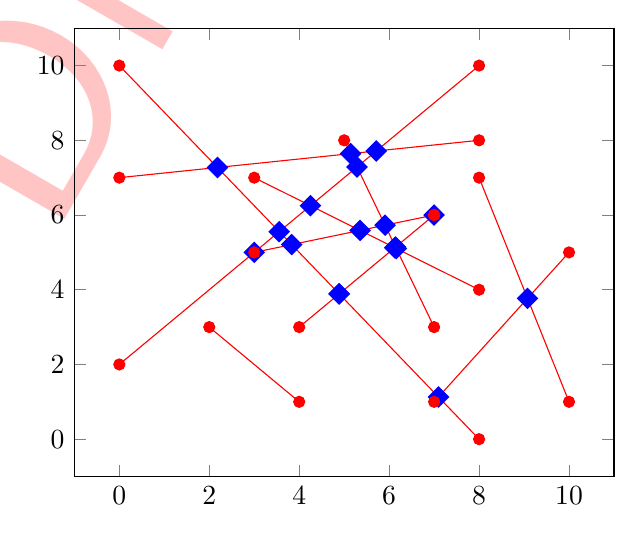
\begin{tikzpicture}
    \begin{axis}
        % Segments
        
            \addplot[red, mark=*] coordinates {(4, 3) (7, 6)};
        
            \addplot[red, mark=*] coordinates {(3, 5) (7, 6)};
        
            \addplot[red, mark=*] coordinates {(5, 8) (7, 3)};
        
            \addplot[red, mark=*] coordinates {(7, 1) (10, 5)};
        
            \addplot[red, mark=*] coordinates {(0, 7) (8, 8)};
        
            \addplot[red, mark=*] coordinates {(8, 7) (10, 1)};
        
            \addplot[red, mark=*] coordinates {(0, 2) (8, 10)};
        
            \addplot[red, mark=*] coordinates {(2, 3) (4, 1)};
        
            \addplot[red, mark=*] coordinates {(3, 7) (8, 4)};
        
            \addplot[red, mark=*] coordinates {(0, 10) (8, 0)};
        
        % Intersections
        
            \node[diamond,fill=blue, inner sep=2pt] at (axis cs:3.5555555555555554, 5.555555555555555) {};
        
            \node[diamond,fill=blue, inner sep=2pt] at (axis cs:4.888888888888889, 3.8888888888888884) {};
        
            \node[diamond,fill=blue, inner sep=2pt] at (axis cs:6.157894736842105, 5.105263157894737) {};
        
            \node[diamond,fill=blue, inner sep=2pt] at (axis cs:4.25, 6.25) {};
        
            \node[diamond,fill=blue, inner sep=2pt] at (axis cs:2.1818181818181817, 7.272727272727273) {};
        
            \node[diamond,fill=blue, inner sep=2pt] at (axis cs:4.888888888888889, 3.888888888888889) {};
        
            \node[diamond,fill=blue, inner sep=2pt] at (axis cs:7.096774193548387, 1.129032258064516) {};
        
            \node[diamond,fill=blue, inner sep=2pt] at (axis cs:3.8333333333333335, 5.208333333333333) {};
        
            \node[diamond,fill=blue, inner sep=2pt] at (axis cs:5.142857142857143, 7.642857142857143) {};
        
            \node[diamond,fill=blue, inner sep=2pt] at (axis cs:5.714285714285714, 7.714285714285714) {};
        
            \node[diamond,fill=blue, inner sep=2pt] at (axis cs:6.142857142857142, 5.142857142857143) {};
        
            \node[diamond,fill=blue, inner sep=2pt] at (axis cs:7.0, 6.0) {};
        
            \node[diamond,fill=blue, inner sep=2pt] at (axis cs:6.125, 5.125) {};
        
            \node[diamond,fill=blue, inner sep=2pt] at (axis cs:5.909090909090909, 5.7272727272727275) {};
        
            \node[diamond,fill=blue, inner sep=2pt] at (axis cs:5.285714285714286, 7.285714285714286) {};
        
            \node[diamond,fill=blue, inner sep=2pt] at (axis cs:9.076923076923077, 3.769230769230769) {};
        
            \node[diamond,fill=blue, inner sep=2pt] at (axis cs:5.352941176470589, 5.588235294117647) {};
        
            \node[diamond,fill=blue, inner sep=2pt] at (axis cs:3.0, 5.0) {};
        
    \end{axis}
\end{tikzpicture}

    \vfill
    \rule{\linewidth}{0.5mm} \\[1cm]
    {\Huge \textsc{\textcolor{fib_red}{Implementation of Sweep Lines}}}\\[1cm]
    {\Large \textsc{Assignment}}\\[0.4cm]
    {\huge \textsc{\textbf{Advanced data structures}}}\\[1cm]
    {\Large \textsc{Master in Research and Innovation - UPC}}\\[0.4cm]
    \rule{\linewidth}{0.5mm} \\[1.5cm]
\end{center}

\vfill

\textbf{Author:}
\begin{itemize}
\item Pierre \textsc{Jézégou}\newline
\textit{(Engineering student at École Centrale de Lille, Exchange student at UPC)}
\end{itemize}

\newpage
\color{black}
\pagecolor{white}
\pagestyle{fancy}
\tableofcontents

\section{Introduction}
\subsection{Sweep lines}
The Segment Intersection Problem is a classic problem in computational geometry. It involves finding all the intersections between a set of line segments in the plane. This problem has various applications, such as in computer graphics, robotics, and geographic information systems.\\

There are several algorithms to solve the Segment Intersection Problem, and one popular approach is the Sweep Line Algorithm. This algorithm involves sweeping a vertical line across the plane and processing the line segments as they are encountered by the sweep line.
To implement the Sweep Line Algorithm, we need to define the data structures and events that will be used. The data structures typically include a status structure to store the line segments that intersect the current sweep line position, and a priority queue to handle the events.\\
The events in the Sweep Line Algorithm correspond to the endpoints of the line segments. As the sweep line encounters an endpoint, it triggers an event that updates the status structure and performs any necessary computations.\\

By implementing the Sweep Line Algorithm, we can efficiently find all the intersections between the line segments and solve the Segment Intersection Problem.


\subsection{Project information}
All the source code (programs, documentation and image generators) is available in the GitHub respository dedicated to the project: https://github.com/pierre-jezegou/sweep-lines

For performance testing of algorithms, we use a MacBook Air with the M2 processor. This hardware provides ample computing power to execute our algorithms efficiently, ensuring swift analysis of their performance. As recommended, this report has been written in \LaTeX.

\section{Sweep Line Algorithm implementation}
\subsection{Structures}
To implement the Sweep Line Algorithm, we need to define the data structures that will be used. First, as the problem is in 2D, we need to define the Point and Segment classes. The Point class represents a point in the plane, while the Segment class represents a line segment defined by two endpoints.\\

The main data structures include the status structure and the event queue. The status structure stores the line segments that intersect the current sweep line position, while the event queue handles the events corresponding to the endpoints of the line segments.

\subsubsection{Point}
First of all, you have to define the \code{Point} class to represent a point in the plane. The Point class has two attributes, $x$ and $y$, representing the $x$ and $y$ coordinates of the point, respectively.
\begin{itemize}
    \item \code{x} (type: \type{float}): $x$ coordinate of the point.
    \item \code{y} (type: \type{float}): $y$ coordinate of the point.
\end{itemize}
\begin{figure}[h]
    \centering
    \begin{tikzpicture}
        \node[draw, rounded corners=2mm, inner sep = 0.2cm, fill=orange!0] { 
        \begin{tikzpicture} 
            \node[inner sep = 1mm] (title) { \Large{\bfseries Point }}; 
            % \draw (title.south west) -- (title.south east);
            \node[at=(title.south), anchor=north, inner sep=3mm, align=left, fill=green!30!black!10, yshift=-0.2cm] (attributes) {
                \begin{minipage}{60mm}
                    \textbf{Attributes}\\
                    \small{0}: \verb|x|\\
\small{1}: \verb|y|
                \end{minipage} 
                };
            % \draw (attributes.north west) -- (attributes.north east);
            \node[at=(attributes.south), anchor=north, inner sep=3mm, align=left, fill=blue!10, yshift=-0.2cm] (methods) {
                \begin{minipage}{60mm}
                    \textbf{Methods}\\
                    \small{0}: \verb|__eq__|\\
\small{1}: \verb|__hash__|\\
\small{2}: \verb|__init__|\\
\small{3}: \verb|__lt__|\\
\small{4}: \verb|__repr__|\\
\small{5}: \verb|format_point|\\
\small{6}: \verb|format_point_segment_pgf|
                \end{minipage} 
                };
            % \draw (methods.north west) -- (methods.north east);
        \end{tikzpicture}
        }; 
    \end{tikzpicture}
    \caption{Class description - Point }
    \label{class:Point}
\end{figure}
I also implemented classic methods to compare two points (\code{__lt__}, \code{__eq__}) or other to represent the point in pgf format.
\subsubsection{Segment}
The \code{Segment} class represents a line segment defined by two endpoints. The Segment class has two attributes, \code{start} and \code{end}, representing the two endpoints of the segment. I also implemented the \code{__lt__} method to compare two segments based on their $x$ and $y$ coordinates. Finally, there is a method to generate the code to represent the segment in pgf format
\begin{itemize}
    \item \code{start} (type: \type{Point}): Start point of the segment.
    \item \code{end} (type: \type{Point}): End point of the segment.
\end{itemize}
\begin{figure}[h]
    \centering
    \begin{tikzpicture}
        \node[draw, rounded corners=2mm, inner sep = 0.2cm, fill=orange!0] { 
        \begin{tikzpicture} 
            \node[inner sep = 1mm] (title) { \Large{\bfseries Segment }}; 
            % \draw (title.south west) -- (title.south east);
            \node[at=(title.south), anchor=north, inner sep=3mm, align=left, fill=green!30!black!10, yshift=-0.2cm] (attributes) {
                \begin{minipage}{60mm}
                    \textbf{Attributes}\\
                    \small{0}: \verb|start|\\
\small{1}: \verb|end|
                \end{minipage} 
                };
            % \draw (attributes.north west) -- (attributes.north east);
            \node[at=(attributes.south), anchor=north, inner sep=3mm, align=left, fill=blue!10, yshift=-0.2cm] (methods) {
                \begin{minipage}{60mm}
                    \textbf{Methods}\\
                    \small{0}: \verb|__eq__|\\
\small{1}: \verb|__init__|\\
\small{2}: \verb|__lt__|\\
\small{3}: \verb|__repr__|\\
\small{4}: \verb|current_y|\\
\small{5}: \verb|segment_to_pgf|
                \end{minipage} 
                };
            % \draw (methods.north west) -- (methods.north east);
        \end{tikzpicture}
        }; 
    \end{tikzpicture}
    \caption{Class description - Segment }
    \label{class:Segment}
\end{figure}

\subsubsection{Event}
As the sweep line encounters the endpoints of the line segments, it triggers events that update the status structure and perform any necessary computations. The Event class represents an event corresponding to an endpoint of a line segment. The Event class has three attributes:
\begin{itemize}
    \item \code{point} (type: \type{Point}): The point corresponding to the event.
    \item \code{segment} (type: \type{Segment}): The segment corresponding to the event.
    \item \code{type} (type: \type{str}): The type of the event, either "start" or "end".
\end{itemize}
There is one more attribute to store the two segments in case of an intersection event.
\begin{figure}[h]
    \centering
    \begin{tikzpicture}
        \node[draw, rounded corners=2mm, inner sep = 0.2cm, fill=orange!0] { 
        \begin{tikzpicture} 
            \node[inner sep = 1mm] (title) { \Large{\bfseries Event }}; 
            % \draw (title.south west) -- (title.south east);
            \node[at=(title.south), anchor=north, inner sep=3mm, align=left, fill=green!30!black!10, yshift=-0.2cm] (attributes) {
                \begin{minipage}{60mm}
                    \textbf{Attributes}\\
                    \small{0}: \verb|point|\\
\small{1}: \verb|segment|\\
\small{2}: \verb|event_type|\\
\small{3}: \verb|intersection_segments|
                \end{minipage} 
                };
            % \draw (attributes.north west) -- (attributes.north east);
            \node[at=(attributes.south), anchor=north, inner sep=3mm, align=left, fill=blue!10, yshift=-0.2cm] (methods) {
                \begin{minipage}{60mm}
                    \textbf{Methods}\\
                    \small{0}: \verb|__eq__|\\
\small{1}: \verb|__hash__|\\
\small{2}: \verb|__init__|\\
\small{3}: \verb|__lt__|\\
\small{4}: \verb|__repr__|
                \end{minipage} 
                };
            % \draw (methods.north west) -- (methods.north east);
        \end{tikzpicture}
        }; 
    \end{tikzpicture}
    \caption{Class description - Event }
    \label{class:Event}
\end{figure}

\subsubsection{Status and EventQueue}
In the implementation of the sweep line algorithm to find intersection points of line segments, I chose to use a heap for the event queue and a \code{SortedList} for the active segments to optimize performance and ensure efficient data management.\\

The heap, implemented using Python's \code{heapq} module, is ideal for the event queue because it allows for efficient extraction of the smallest element, which corresponds to the next event in the sweep line process. The heap provides $O(\log n)$ time complexity for both insertion and extraction, which is crucial for maintaining performance as we dynamically add and remove events.\\

For the active segments, the \code{SortedList} from the \code{sortedcontainers} module is used because it maintains the segments in a sorted order based on their y-coordinates at the current x-coordinate of the sweep line. This is essential for quickly finding and updating the relative order of segments, detecting intersections, and handling segment endpoints efficiently. The \code{SortedList} supports $O(\log n)$ insertion, deletion, and search operations, which significantly enhances the algorithm's efficiency compared to a naive list implementation.\\

By using a heap for the event queue and a \code{SortedList} for the active segments, the sweep line algorithm can efficiently manage the dynamic nature of events and maintain the correct order of segments, leading to an overall optimal performance in detecting intersections.


\section{Intersection}
To compute the intersection of two line segments, I define a function \code{segment_intersection(segment1, segment2)} that uses the parametric form of the segments. Each segment is represented by its start and end points. Let $(x_1, y_1)$ and $(x_2, y_2)$ be the coordinates of the start and end points of $\mathbf{P}$, the first segment, and $(x_3, y_3)$ and $(x_4, y_4)$ be the coordinates of the start and end points of $\mathbf{Q}$, the second segment.

Using the parametric equations:
$$\mathbf{P}(t) = (x_1 + t(x_2 - x_1), y_1 + t(y_2 - y_1))$$
$$\mathbf{Q}(u) = (x_3 + u(x_4 - x_3), y_3 + u(y_4 - y_3))$$

We find the intersection by solving:
$$\left\{\begin{array}{l}
    x_1 + t(x_2 - x_1) = x_3 + u(x_4 - x_3)\\
    y_1 + t(y_2 - y_1) = y_3 + u(y_4 - y_3)
\end{array}\right.$$

The determinant of the system is and if it is equal to 0, the lines are parallel and the function returns \code{False}. Otherwise, we compute the parameters $t$ and $u$:
$$\text{det} = (x_1 - x_2) \cdot (y_3 - y_4) - (y_1 - y_2) \cdot (x_3 - x_4)$$
If $\text{det} = 0$, the lines are parallel, and the function returns \code{False}.

If the lines are not parallel, we compute the parameters $t$ and $u$:
$$t = \frac{(x_1 - x_3) \cdot (y_3 - y_4) - (y_1 - y_3) \cdot (x_3 - x_4)}{\text{det}}$$
$$u = -\frac{(x_1 - x_2) \cdot (y_1 - y_3) - (y_1 - y_2) \cdot (x_1 - x_3)}{\text{det}}$$

The intersection point is valid if $0 \leq t \leq 1$ and $0 \leq u \leq 1$. The intersection coordinates are:
$$
\text{Point} = 
\begin{pmatrix}
    x_1 + t \cdot (x_2 - x_1)\\
    y_1 + t \cdot (y_2 - y_1)
\end{pmatrix}
$$

The function returns this intersection point as a \code{Point} object, rounded to five decimal places. If $t$ and $u$ are not within $[0, 1]$, the function returns \code{False}. Using the parametric form ensures an accurate computation of the intersection.


\subsection{Event driven}
\subsection{Structures used}

\section{Tests and results}
\subsection{Examples implementation}
\subsubsection{First example}
\subsubsection{Second example}
\subsection{Performance tests}
\subsection{Results}

\section{Conclusions}
\section{Appendix}
\lstinputlisting[firstline=1,lastline=50, language=Python]{../additional_algorithms/graphic_sweep_lines.py}

\newpage
\listoffigures
\lstlistoflistings
\listoftables

\input{../random_segments_2.tex}
\input{../tikz.tex}

\end{document}
